\documentclass[conference]{IEEEtran}
\usepackage{graphicx}
\usepackage{booktabs}
\usepackage{amsmath,amssymb}
\usepackage{xcolor}
\usepackage[hidelinks]{hyperref}
\usepackage{cite}

\newcommand{\pending}[1]{\textcolor{red}{[PENDING: #1]}}
\newcommand{\cncm}{C-NCM}

\title{Will It Fall? Diffusion and Flow-Matching World Models Underestimate the Risk of Failure}
\author{\IEEEauthorblockN{Anonymous Authors}}

\begin{document}
\maketitle

\begin{abstract}
World models let a robot imagine what might happen before it acts. Many recent world
models are diffusion or flow-matching models that sample possible futures. For safety,
one of the most useful things such a model can tell us is how likely a failure is. We
test this directly. We simulate a Unitree Go2 quadruped walking on varied terrain while
random pushes hit it. At 1,149 test states we fork the simulator 128 times, so we know
the true probability that the robot falls in the next two seconds. We find two problems.
First, a common logging choice, stopping the log shortly after a fall, hides almost all
early falls from the model and halves the predicted risk. Second, even with clean data and
64 sampling steps, diffusion and flow-matching world models predict only 57\% and 65\% of
the true risk at uncertain states. More sampling steps close this gap only slowly: with
512 steps they still predict 77\% and 83\%. A classifier trained on the same data with the
same network is nearly unbiased (92\%). A coarse-to-fine model that first samples a rough
version of the future and then adds detail, a continuous form of next-concept modeling
(\cncm{}), removes the bias (105\%, 95\% CI 95--117\%), and with only 96 network passes it
already matches what flow matching reaches with 512. The gain is in overall calibration, not in
ranking: all models, including the classifier, rank states equally well, and simple
recalibration on held-out data closes the gap. The main test was pre-registered.
\end{abstract}

% ---------------------------------------------------------------------------------------
\section{Introduction}

A robot that plans with a learned world model needs to know when a plan could end badly.
Think of a quadruped climbing stairs that is about to be pushed. It may catch itself, or
it may fall. A useful world model should not only produce futures that look right. It
should also produce falls about as often as they really happen. If it shows falls too
rarely, a planner that trusts it will take risks it does not see.

Diffusion~\cite{ho2020ddpm,song2021sde} and flow matching~\cite{lipman2023flow,liu2023rectified}
are now common choices for world models and trajectory
models~\cite{janner2022diffuser,alonso2024diamond,ding2024dwm,rigter2024polygrad,valevski2025gamengen}.
They are usually judged by how realistic their samples look or by the error of a single
predicted future. Whether they get \emph{probabilities} right is rarely checked, and for a
good reason: in the real world, and in almost every dataset, each state happens once and
only one future is ever seen. You cannot tell whether a state had a 10\% or a 60\% chance
of failure from one outcome.

Simulation removes this limit. We can copy the full state of the physics engine and the
controller, then run many futures from that exact state that differ only in the random
pushes that will arrive. The fraction of these futures that end in a fall is the true fall
probability of that state. We call this \emph{branching ground truth}. We then ask a world
model for 128 sampled futures from the same state and count how many fall.

With this test we found the following.
\begin{itemize}
  \item \textbf{A data pitfall.} Our first dataset stopped logging one second after each
    fall, a common choice. Because every training window needs two seconds of future,
    windows that start just before a fall were silently dropped. Only 4\% of training
    windows with a fall showed it in the first second, while 51\% of real falls happen
    there (Fig.~\ref{fig:trunc}). This alone halved the predicted risk.
  \item \textbf{A model bias.} With clean data and 64 sampling steps, diffusion and
    conditional flow matching (CFM) still predict only 57\% and 65\% of the true risk at
    uncertain states. Eight times more steps (512) helps but does not close the gap (77\%
    and 83\%). A classifier trained on the same data, with the same inputs and network,
    predicts 92\%. So the bias comes from the generative models, not from the data.
  \item \textbf{A fix.} \cncm{}, a continuous version of next-concept
    modeling~\cite{kumbong2026ncm}, samples a 4-step summary of the future first and then
    adds detail in five more levels. It predicts 105\% of the true risk (95\% CI 95--117\%).
    At equal bias it needs far less compute: 96 network passes give the 83\% that CFM
    needs 512 passes for.
  \item \textbf{Clear limits.} \cncm{} does not rank states better than the other
    models. Every model, including the classifier, reaches about the same per-state
    accuracy (AUC near 0.90), and isotonic recalibration of CFM on held-out data matches
    \cncm{}. Most states that are certain to fall, and that all models miss, are
    deterministic failures of the controller rather than effects of random pushes.
\end{itemize}
We wrote down our hypotheses before running the final test (pre-registration), including
the cases where our method would lose. Two of four hypotheses held. We report all four.

% ---------------------------------------------------------------------------------------
\section{Related Work}

\textbf{World models for robots.} Learned dynamics models have long been used for
planning and policy learning~\cite{chua2018pets,ha2018world,hafner2020dreamer,hafner2025dreamerv3},
including on real robots~\cite{wu2022daydreamer} and legged robots~\cite{li2025rwm}.
More recent models generate whole trajectories or videos with diffusion: Diffuser plans by
denoising trajectories~\cite{janner2022diffuser}, DIAMOND and GameNGen simulate games with
diffusion~\cite{alonso2024diamond,valevski2025gamengen}, and DWM and PolyGRAD predict
multi-step futures for reinforcement learning~\cite{ding2024dwm,rigter2024polygrad}.
Diffusion forcing mixes next-step and full-sequence denoising~\cite{chen2024diffusionforcing}.
These works mostly measure sample quality or downstream return, not whether the
probability of rare outcomes is right.

\textbf{Evaluating world models.} Yu et al.\ argue that world models for embodied
decision-making should be judged by how well they support decisions, with uncertainty
calibration as one of the key axes~\cite{yu2026evaluate}. dWorldEval estimates policy
success rates with a world model and compares them with real execution~\cite{li2026dworldeval}.
Multi-future ground truth exists in other fields: the Garden of Forking Paths gives several
plausible futures for pedestrians~\cite{liang2020garden}, ForecastBench-Sim re-seeds a
strategy game to score forecasts~\cite{lee2026forecastbench}, and Twin Rollouts forks a
simulator to create counterfactual targets for video world models~\cite{ma2026twin}. Our
branches are exact copies of the physics and controller state, and the quantity we score
is the probability of failure.

\textbf{Diffusion, flow matching and rare modes.} Diffusion with a cosine
schedule~\cite{nichol2021improved}, DDIM sampling~\cite{song2021ddim} and flow matching with
a linear path~\cite{lipman2023flow,liu2023rectified,albergo2023interpolants,tong2024cfm}
belong to the same family of Gaussian-path models~\cite{gao2024diffusionflow}, and in our
results they behave alike. Several works report that such models give rare modes too
little mass. SubFlow shows that class-conditional flows trained with a squared loss learn a
frequency-weighted average of sub-modes and neglect rare ones~\cite{lin2026subflow}.
Regional probability matching targets wrong mode frequencies in flow
matching~\cite{huang2026regional}. Other work steers diffusion toward low-density or
minority samples~\cite{sehwag2022low,um2024minority}, and a diffusion model of windstorms
underestimated the most intense events~\cite{tsoi2025windstorms}. Mode interpolation can
also create samples between modes~\cite{aithal2024hallucination}. In a world model the
rare mode is often the failure, which is exactly the outcome a planner must not miss.

\textbf{Coarse-to-fine generation.} Next-scale prediction generates images from coarse to
fine resolution~\cite{tian2024var}, and cascaded diffusion stacks models at growing
resolution~\cite{ho2022cascaded}. Next-concept modeling (NCM) encodes text into a hierarchy
of discrete residual codes and generates one level at a time, all codes of a level in
parallel~\cite{kumbong2026ncm}; its tokenizer uses nested dropout~\cite{rippel2014nested}.
We keep NCM's levels, residuals, attention pattern and corruption, but make every level
continuous and generate it with flow matching.

\textbf{Calibration and failure prediction.} We score probabilities with the Brier
score~\cite{brier1950}, a proper scoring rule~\cite{gneiting2007}. Neural networks are
often miscalibrated~\cite{guo2017calibration}, and isotonic regression is a standard
post-hoc fix~\cite{zadrozny2002,niculescu2005}. Weather forecasting checks the calibration
of diffusion ensembles against observations~\cite{price2025gencast}. In robotics, falls
have been predicted with classifiers~\cite{kalyanakrishnan2011}, and safety critics learn
the chance of future failure~\cite{srinivasan2020safety,thananjeyan2021recovery}.
Recent work models disturbances inside world models for safe
planning~\cite{seo2026latent} or detects failures with a flow-matching world
model~\cite{huang2026fomo}. Counterfactual reasoning with learned models goes back to
structural causal models in policy search~\cite{buesing2019woulda}.

\textbf{Episode ends and censoring.} How an episode ends matters in reinforcement
learning~\cite{pardo2018time}, and many datasets end an episode when the agent
falls~\cite{fu2020d4rl}. Survival analysis has long dealt with outcomes that are cut off
before they are observed~\cite{kaplan1958}. The pitfall in Section~\ref{sec:trunc} is a
selection effect of the same kind, caused by building fixed-length training windows from
episodes that end soon after a failure.

% ---------------------------------------------------------------------------------------
\begin{figure*}[t]
  \centering
  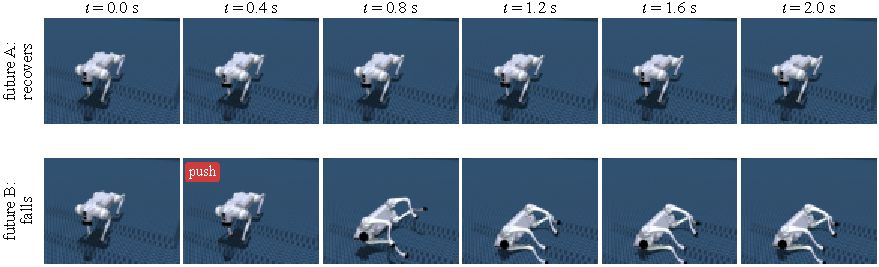
\includegraphics[width=\textwidth]{figs/fig1_fork.pdf}
  \caption{\textbf{One state, two futures.} The robot is simulated up to a moment on
  stairs, then the simulator and controller are copied exactly. Both copies receive the
  same commands. They differ only in the random pushes that arrive later. In future~A the
  robot keeps walking; in future~B a push in the first 0.4\,s makes it fall. Repeating this 128 times
  gives the true fall probability of the starting state (here 34\%). A world model is
  asked for 128 futures from the same state, and we compare how many of them fall.}
  \label{fig:fork}
\end{figure*}

\section{Setup}

\subsection{Robot, controller and terrain}
We use the Unitree Go2 model from MuJoCo Menagerie~\cite{zakka2022menagerie} in
MuJoCo~\cite{todorov2012mujoco}. A model-based controller runs at 50\,Hz: a gait scheduler,
a stance-force balancer that spreads the body wrench over the stance feet by least
squares with friction-cone clipping, Raibert-style foot placement~\cite{raibert1986} and
analytic leg inverse kinematics. Joint PD control with feed-forward torque runs at
500\,Hz, as on the real robot. Each episode lasts 10\,s and has a random terrain type
(flat, rough, slope or stairs), friction (0.4--1.2), payload (0--3\,kg), motor strength
($\pm$10\%), joint damping ($\times$0.7--1.3) and heading. Commands change in random
segments that pick a gait (stand, walk, trot, bound, pace) and a velocity.

\subsection{Random pushes}
Each episode has a push level: none, light, medium or strong. After the first second,
pushes arrive at random times (a Poisson process, 0.4 per second). A push changes the
body's horizontal velocity by up to 0.6, 1.2 or 1.8\,m/s in a random direction and adds a
small random yaw rate. Pushes use their own random number stream, separate from commands,
so we can change the pushes without changing anything else.

\subsection{Prediction task}
The world model gets the current state (46 numbers: base height, gravity direction in the
body frame, body linear and angular velocity, 12 joint angles, 12 joint velocities and the
four foot positions in the body frame), the last 0.5\,s of states, a $7\times7$ height scan
around the robot, a $17\times17$ terrain height map ($\pm$2\,m), the episode parameters and
the planned commands for the next 2\,s. It must predict the next 100 states (2\,s). The
model knows the push level of the episode but not when pushes will come. Those future
pushes are the randomness the model has to represent. A future counts as a \emph{fall} if
the body tilts more than 1\,rad from vertical or the base drops below 0.12\,m at any step.

\subsection{Branching ground truth}
\label{sec:branch}
At an anchor state we copy the MuJoCo state and the full controller state (including gait
phase and internal memory), keep the command random stream, and give each copy a new push
seed. Copies with the same push seed reproduce each other exactly. We run 128 copies for
2\,s and take the fraction that fall as the true fall probability $p$.

The test set has 320 new episodes that were never used before the final run, with four
random anchor times each between 1.5\,s and 7.6\,s (anchors after a fall are skipped),
giving 1,149 anchors. We call an anchor a \emph{fork} when $0.05 < p < 0.95$, meaning the
outcome really depends on the pushes; there are 319 forks, with mean true fall probability
0.164. Anchors in push-free episodes are deterministic ($p$ is exactly 0 or 1). A separate
set of 1,163 anchors from another 320 episodes is used only to fit recalibration maps.

\subsection{Training data}
We generate 6,016 episodes and split them by seed into 4,812 training, 602 validation and
602 test episodes. Training windows start at every step where the robot has not fallen yet
and include the next 100 states, which gives about 1.78 million windows; 6.4\% of them
contain a fall.

\subsection{Metrics}
For each model and anchor we draw 128 futures and take the fraction that fall as the
predicted probability $\hat p$. Our main measure is the \textbf{risk ratio at forks}: the
mean of $\hat p$ over forks divided by the mean of $p$ over forks. A value of 1 means no
overall bias; below 1 means the model underestimates risk. We also report the Brier score
$\frac{1}{n}\sum(\hat p - p)^2$ on forks and on all anchors, the area under the ROC curve
(AUC) with each anchor weighted by $p$ as a fall and $1-p$ as a non-fall, and the energy
distance~\cite{szekely2013energy} between sampled and true futures. Predictions are
averaged over three training seeds. Confidence intervals are 95\% bootstrap intervals over
anchors with 10,000 resamples~\cite{efron1994bootstrap}; differences between models are
paired on the same anchors.

% ---------------------------------------------------------------------------------------
\section{Models}

All world models share one transformer backbone~\cite{vaswani2017attention} (width 256,
4 layers, 4 heads). The inputs become a prefix of tokens and the future becomes 100 tokens,
one per step, each with the planned command of that step. Everything else, including the
training data, steps and optimizer, is the same for all models: 40,000 steps, batch 256,
AdamW~\cite{loshchilov2019adamw} with learning rate $3\times10^{-4}$, a one-cycle schedule,
weight decay 0.01 and gradient clipping at 1. We train three seeds of each model.

\textbf{Diffusion.} Variance-preserving diffusion with a cosine
schedule~\cite{nichol2021improved}; the network predicts the clean future, and we sample
with 64 DDIM steps~\cite{song2021ddim}.

\textbf{CFM.} Flow matching with a straight path between noise and data~\cite{lipman2023flow,liu2023rectified};
the network predicts the clean future, and we sample with 64 Euler steps.

\textbf{\cncm{}.} The future $x$ (100 steps) is split into six levels with lengths
$\ell = (4, 8, 16, 32, 64, 100)$. Let $D_\ell$ average-pool a trajectory in time to $\ell$
steps and $U$ linearly interpolate it back to 100 steps. The levels are residuals:
\begin{equation}
  r_1 = D_{\ell_1}(x), \qquad r_k = D_{\ell_k}\Big(x - \sum_{j<k} U(r_j)\Big),
\end{equation}
so $\sum_k U(r_k) = x$. Level $k$ is a flow-matching model over its $\ell_k$ tokens,
conditioned on the inputs and on all coarser levels, with block-wise attention and a
shared prefix as in NCM~\cite{kumbong2026ncm}. Fig.~\ref{fig:levels} shows how the levels
build up a trajectory. The first level is a 4-step summary of the next two seconds, so
whether the robot ends up on the ground is already visible there. As in NCM, during
training some tokens of the coarser levels are replaced by noise (rates falling linearly
from 0.75 to 0.25 across levels), so that each level learns to tolerate mistakes made by
the levels before it. The loss of level $k$ is weighted by $\ell_k^{1-\alpha}$ with
$\alpha = 0.5$. At test time we sample level by level with 64 Euler steps per level.
Unlike NCM, there is no vector quantization and no categorical distribution; every level
is continuous. With 64 steps per level, \cncm{} uses $6\times64 = 384$ network passes per sample against
64 for CFM; on our GPU (RTX A5000) drawing 128 futures takes 1.9--2.0\,s per anchor with
\cncm{} and 0.73\,s with CFM. Section~\ref{sec:steps} compares the models at equal
numbers of passes.

\textbf{Classifier.} To see whether the inputs hold the information needed to predict a
fall, we train a plain classifier with the same encoders and transformer. A class token
reads the prefix and the planned commands, and the model is trained with log-loss on the
fall label of each training window. Because the terrain map and parameters identify each
training episode, this classifier memorizes training episodes quickly, so we keep the
checkpoint with the lowest log-loss on validation episodes (after 3,500 steps; validation
log-loss 0.188, versus 0.259 for a constant prediction).

\begin{figure*}[t]
  \centering
  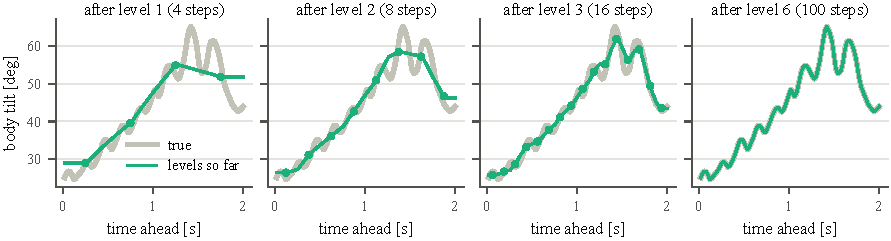
\includegraphics[width=\textwidth]{figs/fig2_levels.pdf}
  \caption{\textbf{How \cncm{} builds a future.} Body tilt over a 2\,s window that ends in
  a fall (gray), and the sum of the levels generated so far (green). Level~1 has only four
  values but already shows the large rise in tilt. Later levels add the faster motion.
  After all six levels the trajectory is exact.}
  \label{fig:levels}
\end{figure*}

% ---------------------------------------------------------------------------------------
\section{A Data Pitfall: Logging Stops After a Fall}
\label{sec:trunc}

Our first dataset stopped logging 50 steps (1\,s) after a fall, which saves space and is
a common choice. Each training window, however, needs 100 future steps. A window that
starts less than 50 steps before a fall would run past the end of the log, so it is never
created. As a result, only 4\% of the training windows that contain a fall show the fall
in the first second of the window, while 51\% of the real falls in our test forks happen
in the first second (Fig.~\ref{fig:trunc}). The models learn that a fall rarely happens
soon, and they predict far too little risk: CFM and diffusion trained on this data
predict 36\% and 31\% of the true risk at forks, about half of what the same models predict
after the fix (Fig.~\ref{fig:ratio}).

We fixed the generator to log 100 steps after a fall and regenerated all 6,016 training
episodes from the same seeds. All states before each fall are identical to the old data
(largest difference 0), so the only change is the longer tail. Our data loader now refuses
data whose tail after a fall is shorter than the model horizon. All results below use
the fixed data unless we say otherwise.

The lesson is general. Any dataset that ends episodes at a failure, or soon after it,
under-represents early failures in fixed-length windows unless the windows are built with
care, for example by padding with the post-failure state. Our earlier pre-registered test
on the truncated data (Appendix~\ref{app:v2}) passed all its hypotheses, including a
per-state accuracy gain for \cncm{}; that accuracy gain did not survive the fix. We
report it to show how easily such a pitfall can produce convincing but wrong results.

\begin{figure}[t]
  \centering
  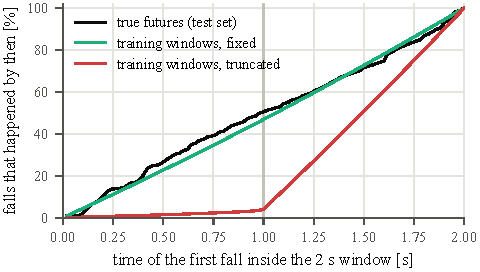
\includegraphics[width=\columnwidth]{figs/fig4_truncation.pdf}
  \caption{\textbf{The logging pitfall.} For falls inside a 2\,s window, the share that
  happened by each time. Real falls (black) are spread over the window, and half of them
  happen in the first second. When logging stops 1\,s after a fall (red), windows that
  start just before a fall are never created, so models almost never see a fall in the
  first second. Logging 100 steps after a fall (green) fixes this.}
  \label{fig:trunc}
\end{figure}

% ---------------------------------------------------------------------------------------
\section{Results}

\subsection{Pre-registered test}
Before the final run we wrote down four hypotheses and the analysis plan (Appendix~\ref{app:prereg}):
\begin{itemize}
  \item[H1] CFM and diffusion underestimate risk at forks even with clean data (upper end of
    the ratio CI below 0.8).
  \item[H2] \cncm{} is less biased than CFM (CI of the ratio difference above 0).
  \item[H3] \cncm{} has a lower fork Brier score than CFM.
  \item[H4] \cncm{} has a lower fork Brier score than CFM after isotonic recalibration.
\end{itemize}
H1 and H2 hold; H3 and H4 do not. Table~\ref{tab:main} and Fig.~\ref{fig:ratio} give the
numbers. CFM predicts 65\% of the true risk at forks (95\% CI 57--74\%) and diffusion 57\%
(50--65\%). \cncm{} predicts 105\% (95--117\%); its ratio is 0.40 higher than CFM's
(CI 0.34--0.47). Fig.~\ref{fig:example} shows one fork: 44 of 128 true futures fall, CFM
samples 18 falls, diffusion 12 and \cncm{} 46.

\begin{table*}[t]
  \centering
  \caption{Main results on the 1,149 test anchors (319 forks). Ratio: mean predicted over
  mean true fall probability at forks, with 95\% CI. Lower is better for Brier and energy.
  Bottom rows: after isotonic recalibration fit on a separate set of 1,163 anchors.}
  \label{tab:main}
  \small
  \begin{tabular}{lccccc}
\toprule
Model & Ratio at forks & Brier (forks) & Brier (all) & AUC & Energy \\
\midrule
CFM & 0.65 [0.57, 0.74] & 0.0246 & 0.0196 & 0.899 & 0.373 \\
Diffusion & 0.57 [0.50, 0.65] & 0.0254 & 0.0209 & 0.894 & 0.372 \\
C-NCM (ours) & 1.05 [0.95, 1.17] & 0.0274 & 0.0209 & 0.902 & 0.431 \\
Classifier & 0.92 [0.82, 1.04] & 0.0271 & 0.0218 & 0.881 & -- \\
\midrule
CFM + isotonic & 1.09 & 0.0245 & 0.0176 & -- & -- \\
Diffusion + isotonic & 1.12 & 0.0290 & 0.0183 & -- & -- \\
C-NCM (ours) + isotonic & 1.11 & 0.0248 & 0.0208 & -- & -- \\
\bottomrule
\end{tabular}

\end{table*}

\begin{figure}[t]
  \centering
  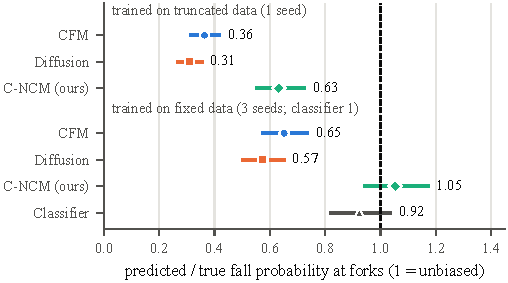
\includegraphics[width=\columnwidth]{figs/fig5_ratio.pdf}
  \caption{\textbf{Risk ratio at forks} (mean predicted over mean true fall probability,
  95\% CI). Top: models trained on the truncated data. Bottom: the same models trained on
  the fixed data, and a classifier with the same inputs and network. Diffusion and CFM
  underestimate risk in both cases; \cncm{} is unbiased on the fixed data.}
  \label{fig:ratio}
\end{figure}

\begin{figure*}[t]
  \centering
  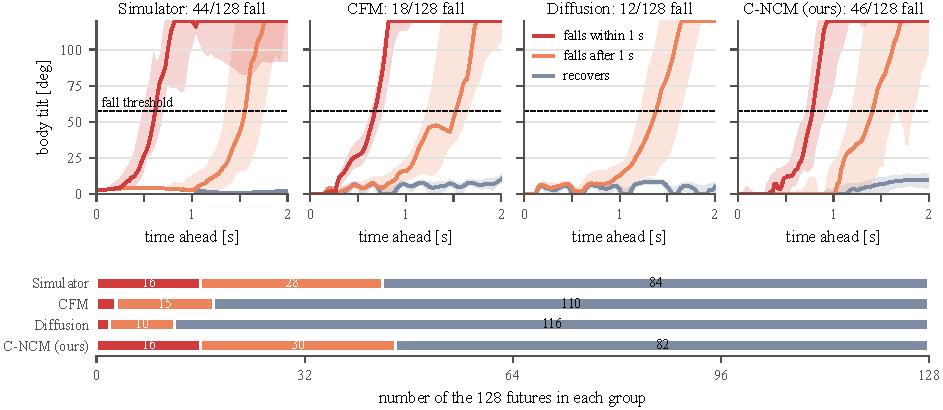
\includegraphics[width=\textwidth]{figs/fig3_example.pdf}
  \caption{\textbf{One fork state} (stairs, strong pushes). Body tilt of 128 futures from the
  simulator and 128 samples from each model (seed 0). Red lines end in a fall. The
  simulator gives 44 falls; CFM and diffusion give far fewer. \cncm{} gives about the right
  number, but its samples are noisier in the first few steps, which is one reason for its
  worse energy distance.}
  \label{fig:example}
\end{figure*}

\subsection{Calibration across risk levels}
Fig.~\ref{fig:calib} breaks the comparison down by true risk. For anchors with true
probability between 0.05 and 0.5, CFM and diffusion lie below the diagonal; at true risk
0.05--0.2 (265 anchors, mean 0.108) they predict 0.074 and 0.064, while \cncm{} predicts
0.128 and the classifier 0.111. \cncm{} over-predicts slightly at safe anchors
($p<0.05$: 0.015 against a true 0.006). All models fall far short at anchors with
$p > 0.5$, which we look at in Section~\ref{sec:certain}.

\begin{figure}[t]
  \centering
  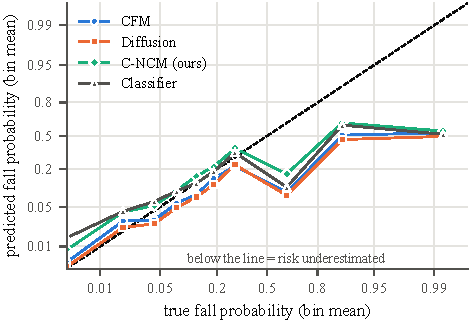
\includegraphics[width=\columnwidth]{figs/fig6_calibration.pdf}
  \caption{\textbf{Calibration by risk level.} Anchors are grouped by true fall
  probability; each point is the mean prediction against the mean truth of a group (logit
  axes). Points below the dashed line underestimate risk.}
  \label{fig:calib}
\end{figure}

\subsection{Per-state accuracy and recalibration}
Getting the average right is not the same as getting each state right. On per-state
accuracy \cncm{} does not win. Its fork Brier score is 0.0274 against 0.0246 for CFM; the
difference, +0.0028, has a CI from $-0.0029$ to $+0.0091$, so we cannot tell them apart.
All three generative models rank anchors equally well (AUC 0.894--0.902). Its energy
distance is worse (0.431 against 0.373), so its sampled trajectories are less accurate in
detail, even though they fall at the right rate.

Because the models rank states equally well, the CFM bias can be removed after training.
An isotonic map from predicted to true probability, fit on the separate calibration set,
brings CFM's fork Brier score to 0.0245, the same as recalibrated \cncm{} (difference
+0.0003, CI $-0.0048$ to $+0.0053$). On all anchors, raw \cncm{} is slightly worse than
recalibrated CFM (+0.0033, CI 0.0007 to 0.0061). Recalibration needs held-out data with
known outcomes and fixes the predicted number, not the sampled futures; \cncm{} gets the
rate right in its samples without extra data. We return to what this means in
Section~\ref{sec:disc}.

\subsection{Is the information in the inputs?}
One explanation for the shared accuracy ceiling would be that generative training throws
away information about falls that the inputs contain. The classifier tests this. It sees
exactly the same inputs and has the same network, but is trained only to predict the fall.
It does not do better: fork Brier 0.0271, AUC 0.881. So, with this data and network size,
the inputs and the amount of data seem to set the limit, not the way the world model is
trained. The classifier is, however, close to unbiased overall (ratio 0.92, CI 0.82--1.04).
This is the key control for our main claim: a model trained on the same data does not
underestimate risk the way diffusion and CFM do, so their bias is not a property of the
data.

\subsection{States that are certain to fall}
\label{sec:certain}
Forty-one anchors fall in at least 95\% of their futures. All models give many of them a
low probability: CFM predicts below 0.4 for 19 of them, diffusion for 22, \cncm{} for 18
and the classifier for 17. Fig.~\ref{fig:certain} shows why these are hard. Nineteen of
the 41 come from push-free episodes, where all 128 futures are identical, and many fall
late in the window (after 1.5\,s) on stairs or slopes. These are failures of the
controller itself, decided by small details of the current state. They are a different
problem from the random forks this paper is about, and no model we tried predicts them
well.

\begin{figure}[t]
  \centering
  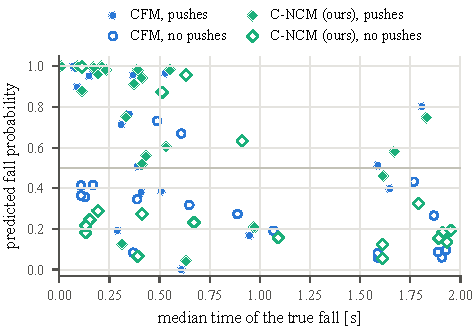
\includegraphics[width=\columnwidth]{figs/fig7_certain.pdf}
  \caption{\textbf{States that are certain to fall} ($p \ge 0.95$, 41 anchors): predicted
  probability against the median time of the true fall. Hollow markers are push-free
  episodes, where all futures are identical. Late, push-free falls are missed by every
  model.}
  \label{fig:certain}
\end{figure}

\subsection{Sampling steps}
\label{sec:steps}
\cncm{} uses more network passes than the flat models (384 against 64), and on the
truncated data we had seen CFM's risk ratio grow with the number of steps. So we checked
whether the flat models simply need more steps. We sampled the seed-0 models again with
16 to 512 steps, and \cncm{} with 16 and 32 steps per level (96 and 192 passes), on the
same test set (Fig.~\ref{fig:steps}).

More steps do help the flat models, but slowly. CFM goes from 0.67 at 64 steps to 0.75,
0.80 and 0.83 at 128, 256 and 512 steps; diffusion goes from 0.57 to 0.67, 0.73 and 0.77.
Each doubling adds less than the one before, and even at 512 steps the upper end of the
CI is below 1 (CFM 0.74--0.93, diffusion 0.68--0.86). \cncm{} reaches 0.83 with 96 passes,
0.97 with 192 and 1.06 with 384. So, at an equal level of bias, \cncm{} needs about five
times fewer passes, and no flat model we ran reached an unbiased ratio. More steps did not
change the per-state picture: CFM's fork Brier score stays at 0.0256--0.0257 from 128 to
512 steps.

This also tells us something about the bias itself. Few steps hurt the rare outcome most:
at 16 steps CFM keeps only 29\% of the true risk. The fall branch seems to be the part of
the distribution that a coarse integration of the flat model loses first.

\begin{figure}[t]
  \centering
  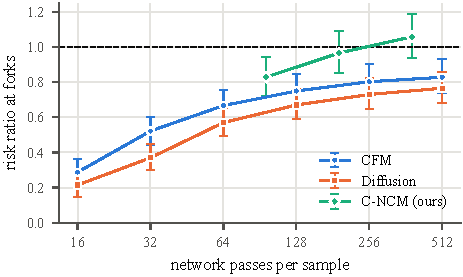
\includegraphics[width=\columnwidth]{figs/fig8_steps.pdf}
  \caption{\textbf{Risk ratio against sampling compute} (seed-0 models, test set, 95\%
  CI). CFM and diffusion use one network pass per step; \cncm{} uses one per step at each
  of its six levels. Flat models improve slowly with more steps and stay biased at 512
  passes; \cncm{} is unbiased from about 200 passes.}
  \label{fig:steps}
\end{figure}

% ---------------------------------------------------------------------------------------
\section{Discussion}
\label{sec:disc}

\textbf{Why would flat models underestimate risk?} We think the answer is in where the
decision to fall is made. A fall is a coarse property of the whole two-second future. A
flat diffusion or flow model makes that choice implicitly, while it denoises all
$100\times46$ numbers at once, and a model trained with a squared loss tends to average
over rare sub-modes~\cite{lin2026subflow}. \cncm{} makes the choice first, on a 4-step
summary where a fall and a recovery look very different, and only then fills in the
detail. The step sweep fits this view: the flat models lose falls first when integration
is coarse, and they recover them only slowly as steps are added. Our ablations on the truncated data agree with this picture: starting from a
4-step level worked better than starting from 16 steps, and removing the residuals or the
corruption reduced the gain (Appendix~\ref{app:v2}). This is a hypothesis that fits our
results, not something we have proven.

\textbf{What does this mean in practice?} If a team has held-out data with known
outcomes, isotonic recalibration of a flat model's fall probability works as well as
\cncm{} for that number. Two things still favor a model that is calibrated by
construction. First, many planners use the sampled futures directly, for example to
average a cost over samples; a recalibrated probability does not change those samples.
Second, recalibration needs outcome data from the same conditions, and a model that is
biased in a predictable way can still be biased in an unpredictable way under new
conditions. We did not test either point, and both deserve a direct test.

\textbf{Limitations.} All results are in simulation, with one robot, one hand-built
controller and one kind of randomness (pushes). The controller has its own failures, which
dominate the states that are certain to fall. We used one network size and one horizon
(2\,s). At the same number of steps per level, \cncm{} is about 2.7 times slower to sample than
CFM in our implementation (though at equal bias it is cheaper), and its trajectories are
less accurate in detail. The step sweep used one seed. The ablations were run before the data fix and
with one seed.

% ---------------------------------------------------------------------------------------
\section{Conclusion}

We measured something world models are rarely tested on: whether they predict failures
as often as failures really happen. Exact branching in simulation gives the answer.
Diffusion and flow-matching world models underestimate the risk of falling. Part of the
gap came from a common logging pitfall, and the rest comes from the models themselves,
since a classifier trained on the same data is nearly unbiased. Adding sampling steps
narrows the gap only slowly. Generating the future
coarse-to-fine with \cncm{} removes the bias, although it does not improve how well states
are ranked. We hope branching ground truth becomes a standard check for world models used
in safety-critical planning.

\bibliographystyle{IEEEtran}
\bibliography{refs}

% ---------------------------------------------------------------------------------------
\appendix

\subsection{Pre-registration}
\label{app:prereg}
The plan was written before any result of the final run. It fixed the training data (the
regenerated 6,016 episodes), the test set (320 new episodes, never generated or looked at
before), the calibration set, the three models and their settings (identical to the
earlier runs), 64 sampling steps and 128 samples, the fork definition, averaging over
three seeds, the bootstrap, the isotonic baseline and hypotheses H1--H4 with their
decision rules. It also fixed the reading in advance: if H1 failed, the earlier
underestimate would be reported as caused by the data pitfall, and a claim that \cncm{} is
better would need both H3 and H4. All secondary measures in this paper (all-anchor Brier,
AUC, energy, calibration bins, the old models on the new test set) were listed there as
``reported regardless of outcome''. The classifier, the analysis of certain-fall states and the sampling-step sweep were
added after the test, as diagnostics.

\subsection{Results on the truncated data and ablations}
\label{app:v2}
Before the data fix we ran a pre-registered test on another fresh set of 1,163 anchors
(316 forks) with three seeds. Ratios were 0.35 (CFM, CI 0.31--0.39), 0.29 (diffusion,
0.25--0.32) and 0.59 (\cncm{}, 0.52--0.67), and \cncm{} had a lower fork Brier score than
CFM ($-0.0037$, CI $-0.0054$ to $-0.0021$). Training CFM twice as long (80k steps) gave
0.34, and \cncm{} without corruption gave 0.45. Table~\ref{tab:ablate} lists the ablations,
all on an exploratory set of 1,170 anchors (280 forks), one seed, 64 steps.

\begin{table}[h]
  \centering
  \caption{Ablations on the truncated data (exploratory set, seed 0, 64 steps).}
  \label{tab:ablate}
  \footnotesize
  \setlength{\tabcolsep}{4pt}
  \begin{tabular}{lccc}
    \toprule
    Model & Ratio & Brier (forks) & Energy \\
    \midrule
    CFM & 0.35 & 0.0339 & 0.358 \\
    CFM, robust normalization & 0.36 & 0.0338 & 0.359 \\
    Diffusion (DDIM) & 0.29 & 0.0375 & 0.358 \\
    Diffusion (ancestral) & 0.17 & 0.0436 & 0.388 \\
    \cncm{}, levels 4--100 (main) & 0.75 & 0.0262 & 0.410 \\
    \quad without residuals & 0.52 & 0.0329 & 0.416 \\
    \quad two levels (4, 100) & 0.56 & 0.0293 & 0.379 \\
    \quad coarsest level 16 (16--100) & 0.49 & 0.0301 & 0.393 \\
    \quad full pyramid (1, 2, \dots, 100) & 1.06 & 0.0357 & 0.430 \\
    Concept-first (k-means) & 0.53 & 0.0511 & 0.519 \\
    \bottomrule
  \end{tabular}
\end{table}

\end{document}
